\documentclass[10pt,conference]{IEEEtran}
\IEEEoverridecommandlockouts

\usepackage{cite}
\usepackage{amsmath,amssymb,amsfonts}
\usepackage{graphicx}
\usepackage{textcomp}
\usepackage{xcolor}
\usepackage{booktabs}
\usepackage{url}
\usepackage{tikz}
\usepackage{pgfplots}
\usetikzlibrary{positioning,shapes.geometric,arrows.meta}
\pgfplotsset{compat=1.18}

\begin{document}

\title{BR-Bench: A Benchmark Linking Continuous Integration Changes to Fault-Revealing Tests}

% Author order is not final; order preserved as requested.
\author{
\IEEEauthorblockN{Prisha Vadhavkar\IEEEauthorrefmark{1}, Sanskriti Singh\IEEEauthorrefmark{1}, Deepanshu\IEEEauthorrefmark{1}\thanks{Author order is provisional and subject to final confirmation before submission.}}
\IEEEauthorblockA{\IEEEauthorrefmark{1}School of Computer Science Engineering and Information Systems\\
Vellore Institute of Technology, Vellore, Tamil Nadu, India\\
\{prisha.vadhavkar2023, sanskriti.singh2023, deepanshu2023\}@vitstudent.ac.in}
}

\maketitle

% [AI DRAFT]
\begin{abstract}
Continuous Integration (CI) services execute automated test suites to detect regressions introduced by pull requests. While industrial platforms at Meta and Google leverage predictive test selection models trained on historical execution data, the research community lacks public, reproducible benchmarks linking pull-request modifications directly to individual failing tests. We present BR-Bench, an open dataset linking code changes to fault-revealing tests mined from GitHub Actions logs across Java and Python open-source repositories. A test is defined as fault-revealing if and only if it fails at the head commit, passes or is absent in the resolved base run, and does not exhibit flakiness across runs on the same commit. The strict benchmark split contains 762 pull-request instances, 4,168 fault-revealing labels, and 2,466 distinct tests across 37 repositories. We evaluate test-to-file binding against pinned commit trees, achieving 94.29\% (5,643/5,985) combined binding and 63.83\% (3,820/5,985) full-confidence fully qualified name binding. In an illustrative application evaluating predictive test selection proxies at $k=10$, historical failure frequency achieves a micro recall of 39.44\% (519/1,316) whereas co-change file mining achieves only 7.67\% (101/1,316). We provide complete raw log archives, extraction pipelines without language model dependencies, and offline reproduction via a single command.
\end{abstract}

\begin{IEEEkeywords}
continuous integration, test selection, regression testing, mining software repositories, fault revelation
\end{IEEEkeywords}

\section{Introduction}

% [AI DRAFT]
Modern software development relies on continuous integration (CI) workflows to catch defects before pull requests merge into shared branches. In CI pipelines, every code modification triggers test suites that consume substantial computational time and energy. Predicting in advance which individual tests are likely to fail on a given pull-request diff would enable teams to run failure-prone tests first, accelerate feedback cycles, and conserve compute resources.

% [AI DRAFT]
Prior academic research addresses neighboring questions rather than empirical test-failure prediction. Change impact analysis (CIA) techniques predict co-changed program entities using version-control history~\cite{borg2017supporting,huang2022change}, capturing developer editing coupling rather than runtime defect propagation. Regression test selection (RTS) tools, such as Ekstazi~\cite{gligoric2015practical} and STARTS~\cite{legunsen2017starts}, compute safe over-approximations of reachable tests via dynamic file or static class dependencies. In contrast, industrial predictive test selection (PTS) systems at Meta~\cite{machalica2019predictive} and Google~\cite{memisevic2023predictive} train statistical models on observed execution outcomes. However, these industrial deployments run on closed-source monorepos, leaving their underlying failure datasets inaccessible to academic researchers.

% [AI DRAFT]
Existing open datasets fail to fill this gap. RTPTorrent~\cite{mattis2020rtptorrent} was mined from Travis CI prior to 2020, covers only Java, organizes data around build jobs rather than pull-request diffs, and emphasizes test prioritization rather than change-to-test fault linking. GHALogs~\cite{moriconi2025ghalogs} provides raw GitHub Actions logs but does not parse granular test outcomes, map tests to source files, or filter non-deterministic executions.

% [AI DRAFT]
To bridge this divide, we present \textsc{BR-Bench}, an open benchmark connecting pull-request file changes directly to the individual test cases that failed because of them. Mined from real GitHub Actions pipelines across 76 swept repositories, \textsc{BR-Bench} extracts structured test outcomes from Gradle, Maven, and pytest execution logs. We resolve base runs on repository histories, filter same-commit test flakiness, and bind test identifiers back to repository source paths.

\section{Data Source and Collection Method}

\begin{figure}[t]
\centering
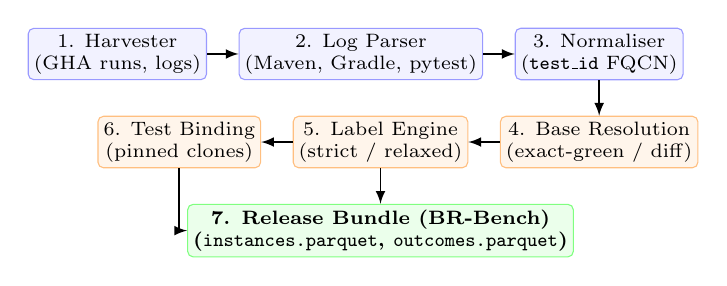
\begin{tikzpicture}[
  node distance=0.45cm and 0.4cm,
  every text node part/.style={align=center},
  box/.style={draw, rectangle, rounded corners=2pt, minimum height=0.6cm, minimum width=1.1cm, font=\scriptsize, inner sep=2pt, fill=black!4},
  proc/.style={box, fill=blue!5, draw=blue!40},
  filter/.style={box, fill=orange!8, draw=orange!50},
  res/.style={box, fill=green!8, draw=green!50, font=\scriptsize\bfseries},
  arr/.style={->, >=latex, semithick}
]
  \node[proc] (harvest) {1. Harvester\\(GHA runs, logs)};
  \node[proc, right=of harvest] (parse) {2. Log Parser\\(Maven, Gradle, pytest)};
  \node[proc, right=of parse] (norm) {3. Normaliser\\(\texttt{test\_id} FQCN)};
  \node[filter, below=of norm] (base) {4. Base Resolution\\(exact-green / diff)};
  \node[filter, left=of base] (label) {5. Label Engine\\(strict / relaxed)};
  \node[filter, left=of label] (bind) {6. Test Binding\\(pinned clones)};
  \node[res, below=of label] (release) {7. Release Bundle (\textsc{BR-Bench})\\(\texttt{instances.parquet}, \texttt{outcomes.parquet})};

  \draw[arr] (harvest) -- (parse);
  \draw[arr] (parse) -- (norm);
  \draw[arr] (norm) -- (base);
  \draw[arr] (base) -- (label);
  \draw[arr] (label) -- (bind);
  \draw[arr] (bind) |- (release);
  \draw[arr] (label) -- (release);
\end{tikzpicture}

\caption{The \textsc{BR-Bench} construction pipeline. Raw CI logs and metadata are harvested, parsed into canonical test identifiers, matched against resolved base runs, filtered for flakiness, bound to source trees, and emitted as Parquet tables.}
\label{fig:pipeline}
\end{figure}

% [AI DRAFT]
The construction pipeline of \textsc{BR-Bench} consists of six reproducible stages (Fig.~\ref{fig:pipeline}): repository selection, metadata harvesting, log parsing, identifier canonicalisation, base-run resolution, and test-to-file binding.

\subsection{Repository Sampling and Harvesting}
% [AI DRAFT]
We selected candidate repositories from the SEART GitHub platform~\cite{dabic2021sampling}. Starting from an export of 3,671 open-source repositories, we retained 2,646 repositories active on GitHub Actions with at least 100 workflow runs in the preceding 90 days. We identified 2,333 repositories executing test-intent workflows (excluding linting or deployment tasks). We sampled 300 repositories into a balanced evaluation frame across Java and Python. A harvester swept 76 repositories before log retention limits intervened (a 77th repository exists in corpus metadata without harvested runs; we report the 76 swept repositories). For each workflow run, the harvester downloaded run metadata, job step statuses, check-run annotations, and raw textual execution logs via the GitHub REST API.

\subsection{Log Parsing and Test Identifier Normalisation}
% [AI DRAFT]
Because GitHub Actions treats test execution as unstructured stdout and stderr streams, test verdicts must be parsed from job logs. We built deterministic line parsers for three major test runners: Maven Surefire/Failsafe, Gradle Test Runner, and pytest. The parsers extract test outcomes (pass, fail, error, skip) and execution durations without relying on external large language models (LLMs). Each parsed test is mapped to a canonical identifier of the format \texttt{module::class::method} for JVM languages and \texttt{filepath::test\_function} for Python. Bare class identifiers are disambiguated using package declarations recovered from logs where available.

\subsection{Base-Run Resolution and Fault Revelation}
% [AI DRAFT]
A test failure at a pull request's head commit does not imply that the pull request caused the failure; the test may have been broken in the upstream base branch. To establish causality, every failed head run must be paired with an appropriate base run. For each pull-request run on head commit $H$ targeting base branch commit $B$, we search repository history for a workflow run on $B$ executing the identical workflow. If a run on $B$ exists and completed with conclusion \texttt{success}, we record an \texttt{exact\_green} resolution. If no run exists on $B$, we traverse ancestor commits along the default branch within a maximum distance of 10 commits.

% [AI DRAFT]
Let $T_{\text{head\_fail}}$ denote tests failing in the head run, $T_{\text{base\_fail}}$ denote tests failing in the resolved base run, and $T_{\text{flaky}}$ denote tests exhibiting flakiness on identical commits. The set of fault-revealing tests $T_{\text{reveal}}$ is defined as:
\begin{equation}
T_{\text{reveal}} = (T_{\text{head\_fail}} \setminus T_{\text{base\_fail}}) \setminus T_{\text{flaky}}.
\end{equation}
Under the \texttt{strict} split, we require that the base run is verified green or that $T_{\text{base\_fail}}$ is fully parsed. Under the \texttt{relaxed} split, runs with missing base logs are retained if the base run concluded with status \texttt{success}.

\subsection{Flakiness Filtering and Test-to-File Binding}
% [AI DRAFT]
Flaky tests flip their status non-deterministically without code changes~\cite{bell2018deflaker}. We detect same-SHA flips across repeated workflow executions on the exact same commit hash. Across 11,557 evaluated (head SHA, workflow, test) groups, 62 instances (0.54\%) flipped, leading to the removal of 46 flaky labels from the relaxed set (1.09\% of 4,214 labels) to form the strict set.

% [AI DRAFT]
To enable change impact analysis, canonical test identifiers must bind to physical test source files. We bind identifiers against pinned repository clones recorded in \texttt{docs/CLONE\_PINS.json} rather than volatile branch heads. Basename-only matches achieve 0.5 confidence, while fully qualified class names that match uniquely achieve 1.0 confidence.

\section{Storage and Schema}

\begin{table}[t]
\caption{Key Schema Fields of \textsc{BR-Bench} Tables}
\label{tab:schemas}
\centering
\scriptsize
\begin{tabular}{llp{3.8cm}}
\toprule
\textbf{Table} & \textbf{Field} & \textbf{Type and Description} \\
\midrule
\texttt{instances} & \texttt{instance\_id} & String; PK: sha256(repo $\vert$ head $\vert$ run) \\
& \texttt{repo} & String; repository (\texttt{owner/name}) \\
& \texttt{language} & String; language (\texttt{java} or \texttt{python}) \\
& \texttt{head\_sha} & String; commit SHA at head \\
& \texttt{base\_sha} & String; target commit on base branch \\
& \texttt{base\_run\_id} & Int64; resolved base run identifier \\
& \texttt{base\_run\_distance} & Int32; commit distance base to head \\
& \texttt{changed\_files} & List$<$Struct$>$; modified paths, diff hunks \\
& \texttt{author\_login} & String; pseudonymised author hash \\
\midrule
\texttt{outcomes} & \texttt{instance\_id} & String; FK into \texttt{instances} \\
& \texttt{test\_id} & String; canonical \texttt{module::class::method} \\
& \texttt{test\_file} & String; repo-relative test path \\
& \texttt{status\_head} & String; outcome at head (\texttt{fail}, \texttt{error}) \\
& \texttt{status\_base} & String; outcome at base (\texttt{pass}, \texttt{absent}) \\
& \texttt{is\_fault\_revealing} & Boolean; fault revelation label \\
& \texttt{same\_sha\_flip} & Boolean; flaky flag on same commit \\
& \texttt{split\_strict} & Boolean; inclusion in strict split \\
& \texttt{binding\_strategy} & String; exact FQCN, basename, unbound \\
\bottomrule
\end{tabular}
\end{table}

% [AI DRAFT]
\textsc{BR-Bench} is published in Apache Parquet format to ensure efficient columnar storage and typed schema enforcement, accompanied by a structured dataset datasheet~\cite{gebru2021datasheets}. Table~\ref{tab:schemas} details the primary fields across the core tables. The \texttt{instances.parquet} table stores pull-request changes, commit hashes, base-run metadata, and file diffs. The \texttt{outcomes.parquet} table records per-test observations, parsed verdicts, flakiness indicators, and ground-truth fault-revelation labels. Auxiliary tables provide historical commit co-change graphs (\texttt{cochange.parquet}) and candidate test spaces (\texttt{candidates.parquet}).

% [AI DRAFT]
To protect contributor privacy, all author usernames are pseudonymised using a salted SHA-256 hash across 1,791 unique authors. Failure messages were scanned for credentials; zero blocking secrets were identified, while 5 review samples were flagged for human verification.

\section{Dataset Overview and Quality}

\subsection{Corpus and Attrition Funnel}

\begin{table}[t]
\caption{Pipeline Attrition Funnel across Stages}
\label{tab:funnel}
\centering
\scriptsize
\begin{tabular}{lrrr}
\toprule
\textbf{Attrition Stage} & \textbf{Count} & \textbf{\% Prev.} & \textbf{\% Total} \\
\midrule
\multicolumn{4}{l}{\textit{Repositories}} \\
SEART GitHub export & 3,671 & --- & 100.00\% \\
CI-live ($\ge 100$ runs in 90 days) & 2,646 & 72.08\% & 72.08\% \\
Test-intent workflow detected & 2,333 & 88.17\% & 63.55\% \\
Sampled into candidate frame & 300 & 12.86\% & 8.17\% \\
Swept by harvester & 76 & 25.33\% & 2.07\% \\
Repositories with $\ge 1$ failed run & 69 & 90.79\% & 1.88\% \\
Repositories with $\ge 1$ strict instance & 37 & 53.62\% & 1.01\% \\
\midrule
\multicolumn{4}{l}{\textit{Workflow Runs}} \\
Total runs discovered & 165,349 & --- & 100.00\% \\
Failed runs & 12,581 & 7.61\% & 7.61\% \\
Failed-job log captured on disk & 6,586 & 52.35\% & 3.98\% \\
Parsed head test failure & 1,774 & 26.94\% & 1.07\% \\
Resolved base run found & 1,348 & 75.99\% & 0.82\% \\
Known base failure set & 897 & 66.54\% & 0.54\% \\
Emitted strict benchmark instances & 762 & 84.95\% & 0.46\% \\
\bottomrule
\end{tabular}
\end{table}

% [AI DRAFT]
The construction of \textsc{BR-Bench} exhibits significant attrition, documented in Table~\ref{tab:funnel}. Of 165,349 workflow runs discovered across 76 swept repositories, 12,581 (7.61\%) failed. However, only 6,586 failed runs had accessible logs on disk due to GitHub Actions' strict 90-day retention window. Only 1,774 runs contained a parseable test failure, and base resolution resolved 1,348 runs. Filtering out unverified base states yields 897 instances with a known base failure set and 762 instances in the strict split.

\subsection{Dataset Composition}

\begin{table}[t]
\caption{Dataset Composition by Benchmark Split and Language}
\label{tab:composition}
\centering
\scriptsize
\begin{tabular}{lrrrrr}
\toprule
\textbf{Split / Lang.} & \textbf{Repos} & \textbf{Instances} & \textbf{Labels} & \textbf{Distinct Tests} \\
\midrule
\textbf{All Split} & \textbf{37} & \textbf{897} (100.0\%) & \textbf{4,384} (100.0\%) & \textbf{2,500} \\
\quad Java & 35 & 767 (85.51\%) & 4,054 (92.47\%) & 2,374 \\
\quad Python & 2 & 130 (14.49\%) & 330 (7.53\%) & 126 \\
\midrule
\textbf{Relaxed Split} & \textbf{37} & \textbf{770} (85.84\%) & \textbf{4,214} (96.12\%) & \textbf{2,484} \\
\quad Java & 35 & 646 (83.90\%) & 3,901 (92.57\%) & 2,359 \\
\quad Python & 2 & 124 (16.10\%) & 313 (7.43\%) & 125 \\
\midrule
\textbf{Strict Split} & \textbf{37} & \textbf{762} (84.95\%) & \textbf{4,168} (95.07\%) & \textbf{2,466} \\
\quad Java & 35 & 638 (83.73\%) & 3,855 (92.49\%) & 2,341 \\
\quad Python & 2 & 124 (16.27\%) & 313 (7.51\%) & 125 \\
\bottomrule
\end{tabular}
\end{table}

% [AI DRAFT]
Table~\ref{tab:composition} details the final composition of \textsc{BR-Bench}. The strict split comprises 762 instances, 4,168 labels, and 2,466 distinct tests across 37 repositories. Java projects represent 83.73\% of strict instances (638/762) and 92.49\% of labels (3,855/4,168), while Python represents 16.27\% of instances (124/762) and 7.51\% of labels (313/4,168).

\subsection{Quality and Verification}

\begin{table}[t]
\caption{Data Quality Indicators and Failure Classification}
\label{tab:quality}
\centering
\scriptsize
\begin{tabular}{llr}
\toprule
\textbf{Dimension} & \textbf{Metric} & \textbf{Value (n/d)} \\
\midrule
Base Resolution & No usable base found & 5,520/12,581 (43.88\%) \\
& Distance median (p90, max) & 0 (2, 10) commits \\
\midrule
Flakiness & Same-SHA flip rate & 62/11,557 (0.54\%) \\
& Flaky labels pruned & 46/4,214 (1.09\%) \\
\midrule
Test Binding & Combined binding rate & 5,643/5,985 (94.29\%) \\
& Full confidence (FQCN) & 3,820/5,985 (63.83\%) \\
& Basename-only confidence & 1,823/5,985 (30.46\%) \\
& Not found / Ambiguous & 178 / 164 (2.97\% / 2.74\%) \\
\midrule
Failure Classes & Code-level assertions & 729/4,168 (17.49\%) \\
(Strict Labels) & Timeout errors & 112/4,168 (2.69\%) \\
& Environment failures & 89/4,168 (2.14\%) \\
& Unknown / unclassified & 3,238/4,168 (77.69\%) \\
\bottomrule
\end{tabular}
\end{table}

% [AI DRAFT]
We report data quality measurements in Table~\ref{tab:quality}. For base resolution, 43.88\% of failed runs (5,520/12,581) lacked a usable base run, primarily because pull requests targeted branches without prior workflow executions. Where resolved, the median commit distance between head and base was 0 commits ($p90=2$, $\max=10$). In test-to-file binding across 5,985 distinct (repo, test) pairs, combined binding achieved 94.29\% (5,643/5,985), while full-confidence binding reached 63.83\% (3,820/5,985).

% [AI DRAFT]
An automated regex audit classified failure messages into four classes: code-level assertions accounted for 17.49\% (729/4,168), timeout errors represented 2.69\% (112/4,168), and strict environment failures (e.g., missing CUDA GPUs or network timeouts) accounted for 2.14\% (89/4,168). A majority of labels (77.69\%, 3,238/4,168) remain unknown due to uncaptured stack traces or unparsed error texts.

\section{How the Data Has Been Used: RQ1 Example}

\begin{figure}[t]
\centering
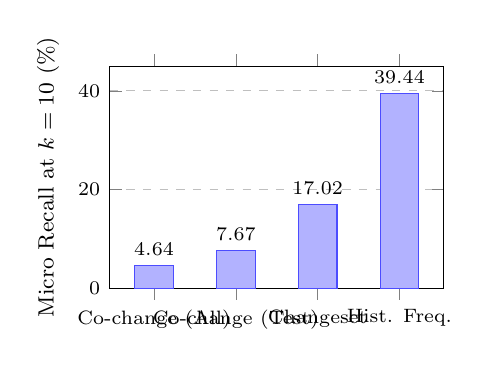
\begin{tikzpicture}
\begin{axis}[
    ybar,
    bar width=14pt,
    width=0.48\textwidth,
    height=4.4cm,
    ymin=0,
    ymax=45,
    ylabel={Micro Recall at $k=10$ (\%)},
    symbolic x coords={Co-change (All), Co-change (Test), Changeset, Hist. Freq.},
    xtick=data,
    nodes near coords,
    nodes near coords align={vertical},
    every node near coord/.append style={font=\scriptsize},
    tick label style={font=\scriptsize},
    label style={font=\footnotesize},
    ymajorgrids=true,
    grid style=dashed,
    enlarge x limits=0.18,
]
\addplot[fill=blue!30, draw=blue!70] coordinates {
    (Co-change (All), 4.64)
    (Co-change (Test), 7.67)
    (Changeset, 17.02)
    (Hist. Freq., 39.44)
};
\end{axis}
\end{tikzpicture}

\caption{Micro recall at $k=10$ across test selection proxies evaluated on \textsc{BR-Bench} ($n=576$ identical instances, 1,316 positive labels).}
\label{fig:rq1}
\end{figure}

% [AI DRAFT]
To demonstrate how \textsc{BR-Bench} serves as an empirical benchmark, we evaluate an example research question (RQ1): \textit{How accurately do conventional change impact analysis proxies and historical baselines identify fault-revealing tests?}

\subsection{Experimental Setup and Leakage Audit}
% [AI DRAFT]
We evaluate four test selection strategies at a budget of $k=10$ candidate files:
\begin{enumerate}
\item \textit{Co-change (All)}: Trailing 365-day co-change partners mined from Git commits.
\item \textit{Co-change (Test Only)}: Co-change restricted to conventional test file patterns (\texttt{src/test/}, \texttt{*Test.java}, \texttt{test\_*.py}).
\item \textit{Changeset Baseline}: Tests living directly within the pull request's modified files.
\item \textit{Historical Frequency}: Tests ranked by historical failure counts in runs strictly prior to the evaluated instance.
\end{enumerate}

% [AI DRAFT]
To prevent temporal data leakage, co-change history was mined strictly prior to each run's start timestamp. An audit revealed that a naive static co-change table leaked future commits in 713/713 audited instances, and an uncorrected historical baseline double-counted failures across multiple splits (224,758 rows for 78,399 distinct labels). After enforcing per-instance trailing windows, symmetric partner lookups, and single-split counting, zero leakage violations remain across all 762 instances.

\subsection{Results}
% [AI DRAFT]
All methods are evaluated on the identical set of $n=576$ instances where the co-change proxy yields predictions ($1,316$ positive test labels; 462 Java, 114 Python). As shown in Fig.~\ref{fig:rq1}, all-partner co-change achieves a micro recall of only 4.64\% (61/1,316; mean P/R/J: 0.011 / 0.051 / 0.010). Restricting co-change to conventional test files improves micro recall to 7.67\% (101/1,316; mean P/R/J: 0.054 / 0.087 / 0.038). The changeset baseline recalls 17.02\% (224/1,316; mean P/R/J: 0.039 / 0.245 / 0.037). In contrast, historical failure frequency achieves 39.44\% micro recall (519/1,316; mean P/R/J: 0.185 / 0.517 / 0.178). Removing environment and timeout failure labels leaves this ordering unchanged. This evaluation demonstrates that historical test failure frequency dramatically outperforms version-control co-change heuristics at identifying true regressions.

\section{Originality and Similar Datasets}

% [AI DRAFT]
\textsc{BR-Bench} differs substantively from existing benchmarks:
\begin{itemize}
\item \textbf{RTPTorrent}~\cite{mattis2020rtptorrent}: While RTPTorrent provides test outcomes from Travis CI for Java, it organizes data by build job rather than pull-request diffs, predates GitHub Actions, and focuses on test prioritization. \textsc{BR-Bench} targets diff-to-failing-test prediction across Java and Python.
\item \textbf{GHALogs}~\cite{moriconi2025ghalogs}: GHALogs provides an archive of raw GitHub Actions logs. However, it does not extract test-level outcomes, link pull-request diffs, resolve base commits, or detect flaky tests. \textsc{BR-Bench} supplies these processed, fault-revealing labels.
\item \textbf{Static and Dynamic RTS Tools}: Tools such as Ekstazi~\cite{gligoric2015practical}, STARTS~\cite{legunsen2017starts}, and Chianti~\cite{ren2004chianti} select tests reaching modified code dynamically or statically. These tools compute safe reachability over-approximations, whereas \textsc{BR-Bench} captures empirical failures during CI runs.
\item \textbf{Industrial PTS Studies}: Industrial studies from Meta~\cite{machalica2019predictive} and Google~\cite{memisevic2023predictive} train predictive models on proprietary monorepos. \textsc{BR-Bench} provides an open dataset enabling the research community to replicate and benchmark predictive test selection techniques.
\end{itemize}

\section{Limitations and Threats}

% [AI DRAFT]
We identify several limitations and threats to validity:
\begin{enumerate}
\item \textit{Pre-registered Sample Size Gates}: Our pre-registered Gate 1 threshold ($\ge 5,000$ strict positives) was \textbf{not met}, reaching 4,168/5,000 labels (83.36\%) and 762/5,000 instances (15.24\%). Furthermore, Gate 1.5 ($\ge 70\%$ test binding) was met on the combined metric (94.29\%, 5,643/5,985) but \textbf{not met} at full-confidence FQCN resolution (63.83\%, 3,820/5,985).
\item \textit{Parser Evaluation}: Parser evaluation figures on our fixture corpus (46/46) and holdout v1 (30/30) were derived from development sets used during parser tuning. Independent parser precision on holdout v5 was \textbf{not measured} [MISSING: blind human annotations on holdout v5 fixtures] due to the lack of completed blind human annotations.
\item \textit{Observational Ground Truth}: Labels represent observational CI execution outcomes rather than causal defect injections or isolated re-executions. Non-test environmental failures remain present in a small minority of labels (2.14\% strict environment, 2.69\% timeout).
\item \textit{90-Day Retention Cliff}: Because GitHub Actions purges raw log artifacts after 90 days, 33.21\% of failed runs (4,458/13,422) had already expired at the time of harvesting. Exact reproduction must rely on our archived raw store rather than live GitHub API calls.
\item \textit{Repository Skew}: The strict benchmark split is dominated by Java repositories (35 Java vs. 2 Python), with high volume from a small set of active projects (e.g., Apache Beam, Stirling-PDF).
\end{enumerate}

\section{Future Research Questions and Improvements}

% [AI DRAFT]
\textsc{BR-Bench} opens promising directions for empirical software engineering research:
\begin{itemize}
\item \textit{Machine Learning for Test Selection}: Researchers can train graph neural networks and language models on code diffs and test paths to predict regressions without execution overhead.
\item \textit{Independent Test Re-execution}: A planned causal subset will execute test suites in isolated containerized environments to distinguish true regressions from environmental flakes.
\item \textit{Multi-Language Expansion}: Future versions will extend coverage to JavaScript, TypeScript, and Go repositories, balancing the language distribution.
\end{itemize}

\section{Availability and Reproducibility}

% [AI DRAFT]
All datasets and extraction scripts are released under open licenses. The processed tables and raw log store are deposited on Zenodo at \texttt{[DOI-DATA]}. The complete source code pipeline is available on GitHub at \texttt{[DOI-CODE]}. The dataset numbers in this paper can be regenerated offline in approximately 8 minutes on a standard laptop by executing \texttt{make tables}, and the test suite comprising 782 automated tests passes cleanly via \texttt{make test}.

\section{Conclusion}

% [AI DRAFT]
We presented \textsc{BR-Bench}, an open benchmark linking pull-request modifications to fault-revealing tests across Java and Python GitHub Actions pipelines. By resolving base runs, filtering same-commit flakiness, and binding tests to source files, \textsc{BR-Bench} provides an empirical ground truth for regression test selection and impact analysis. Our initial evaluation demonstrates that historical test failure frequency substantially outperforms conventional co-change proxies, establishing a foundation for future predictive test selection research.

\newpage
\bibliographystyle{IEEEtran}
\bibliography{refs}

\end{document}
